\title{Conference Report: \emph{Why R?} 2018}
\author{by Micha\l{} Burdukiewicz, Marta Karas, Leon Eyrich Jessen, Marcin Kosi\'{n}ski, Bernd Bischl and Stefan R\"odiger}

\maketitle

\begin{figure}[htbp]
  \centering
  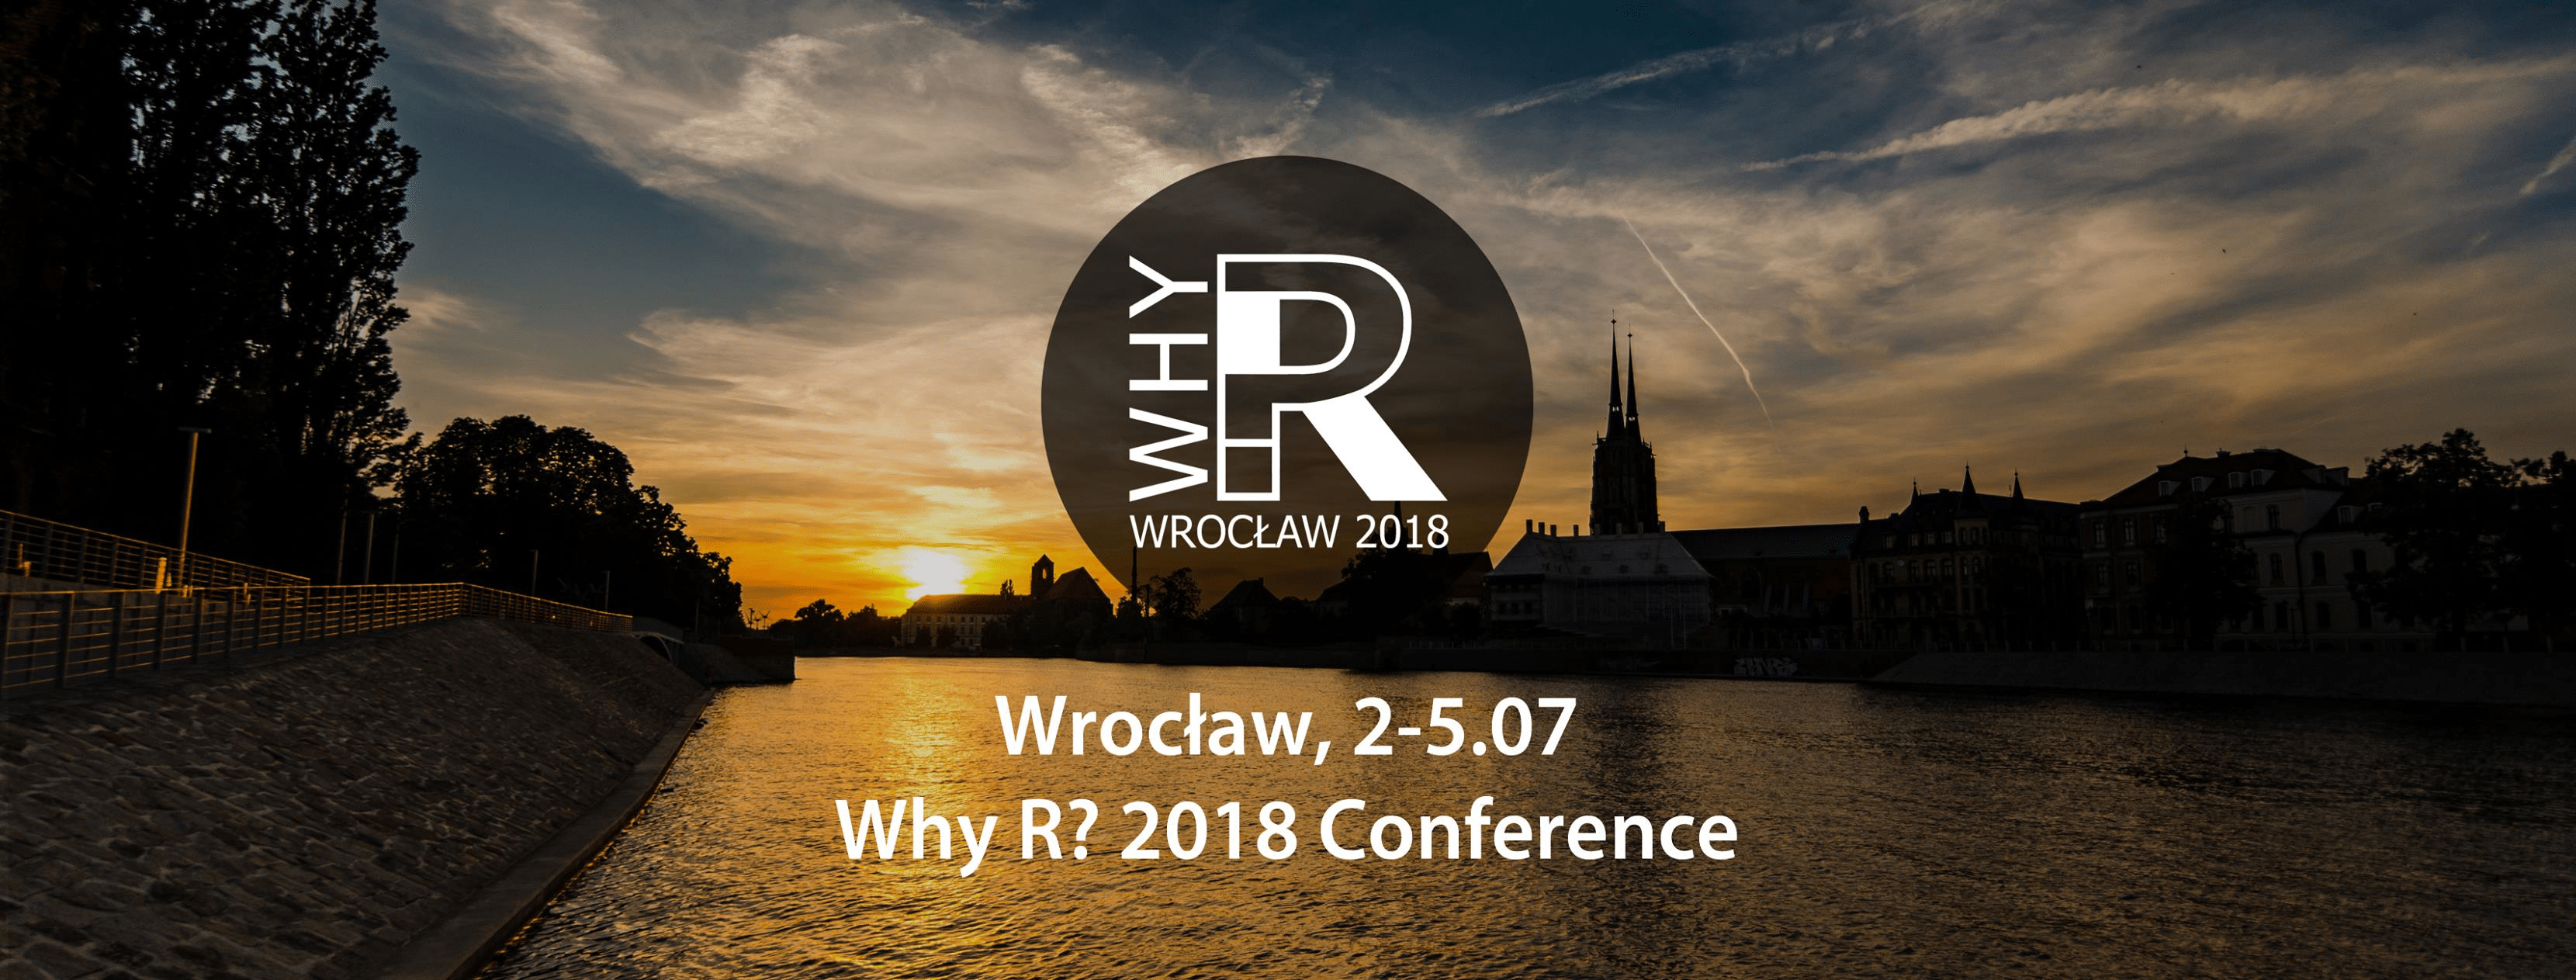
\includegraphics[width=0.8\columnwidth]{whyr_banner}
  \caption{\emph{Why R?} 2018 conference banner used for social media promotion. The background displays banks of the Odra river in Wroclaw -- the city of Poland where the conference was held.}
  \label{figure:whyr_banner}
\end{figure}


%This part will be removed: how to use changes packages. Locate your id in the preamble, and look: \added[id=MB]{I am adding things}, \deleted[id=MB]{removing them} or even try to \replaced[id=MB]{easily}{laboriously} replace something.

\section{\emph{Why R?} 2018 conference}

The primary purpose of the \emph{Why R?} 2018 conference was to provide R programming language enthusiasts with an opportunity to meet and discuss experiences in R software development and analysis applications, for both  academia and industry professionals. The event was held 2-5 August, 2018 in a city of Wroclaw, a strong academic and business center of Poland. The total of approximately 250 people from 6 countries attended the main conference event. Additionally, approximately 540 R users attended the pre-meetings in eleven cities across Europe (Figure~\ref{figure:premeetings}).

~\\ \emph{Why R?} 2018 conference is the continuation of the \emph{Why R?}'s first edition that took place Sep 27-29, 2017 at the Warsaw University of Technology in Warsaw (Poland). Given the success of the first event, this year's conference extended its program concept and scope; importantly, \emph{Why R?} 2018 conference  was held as international. 

\begin{figure}%[htbp]
  \centering
  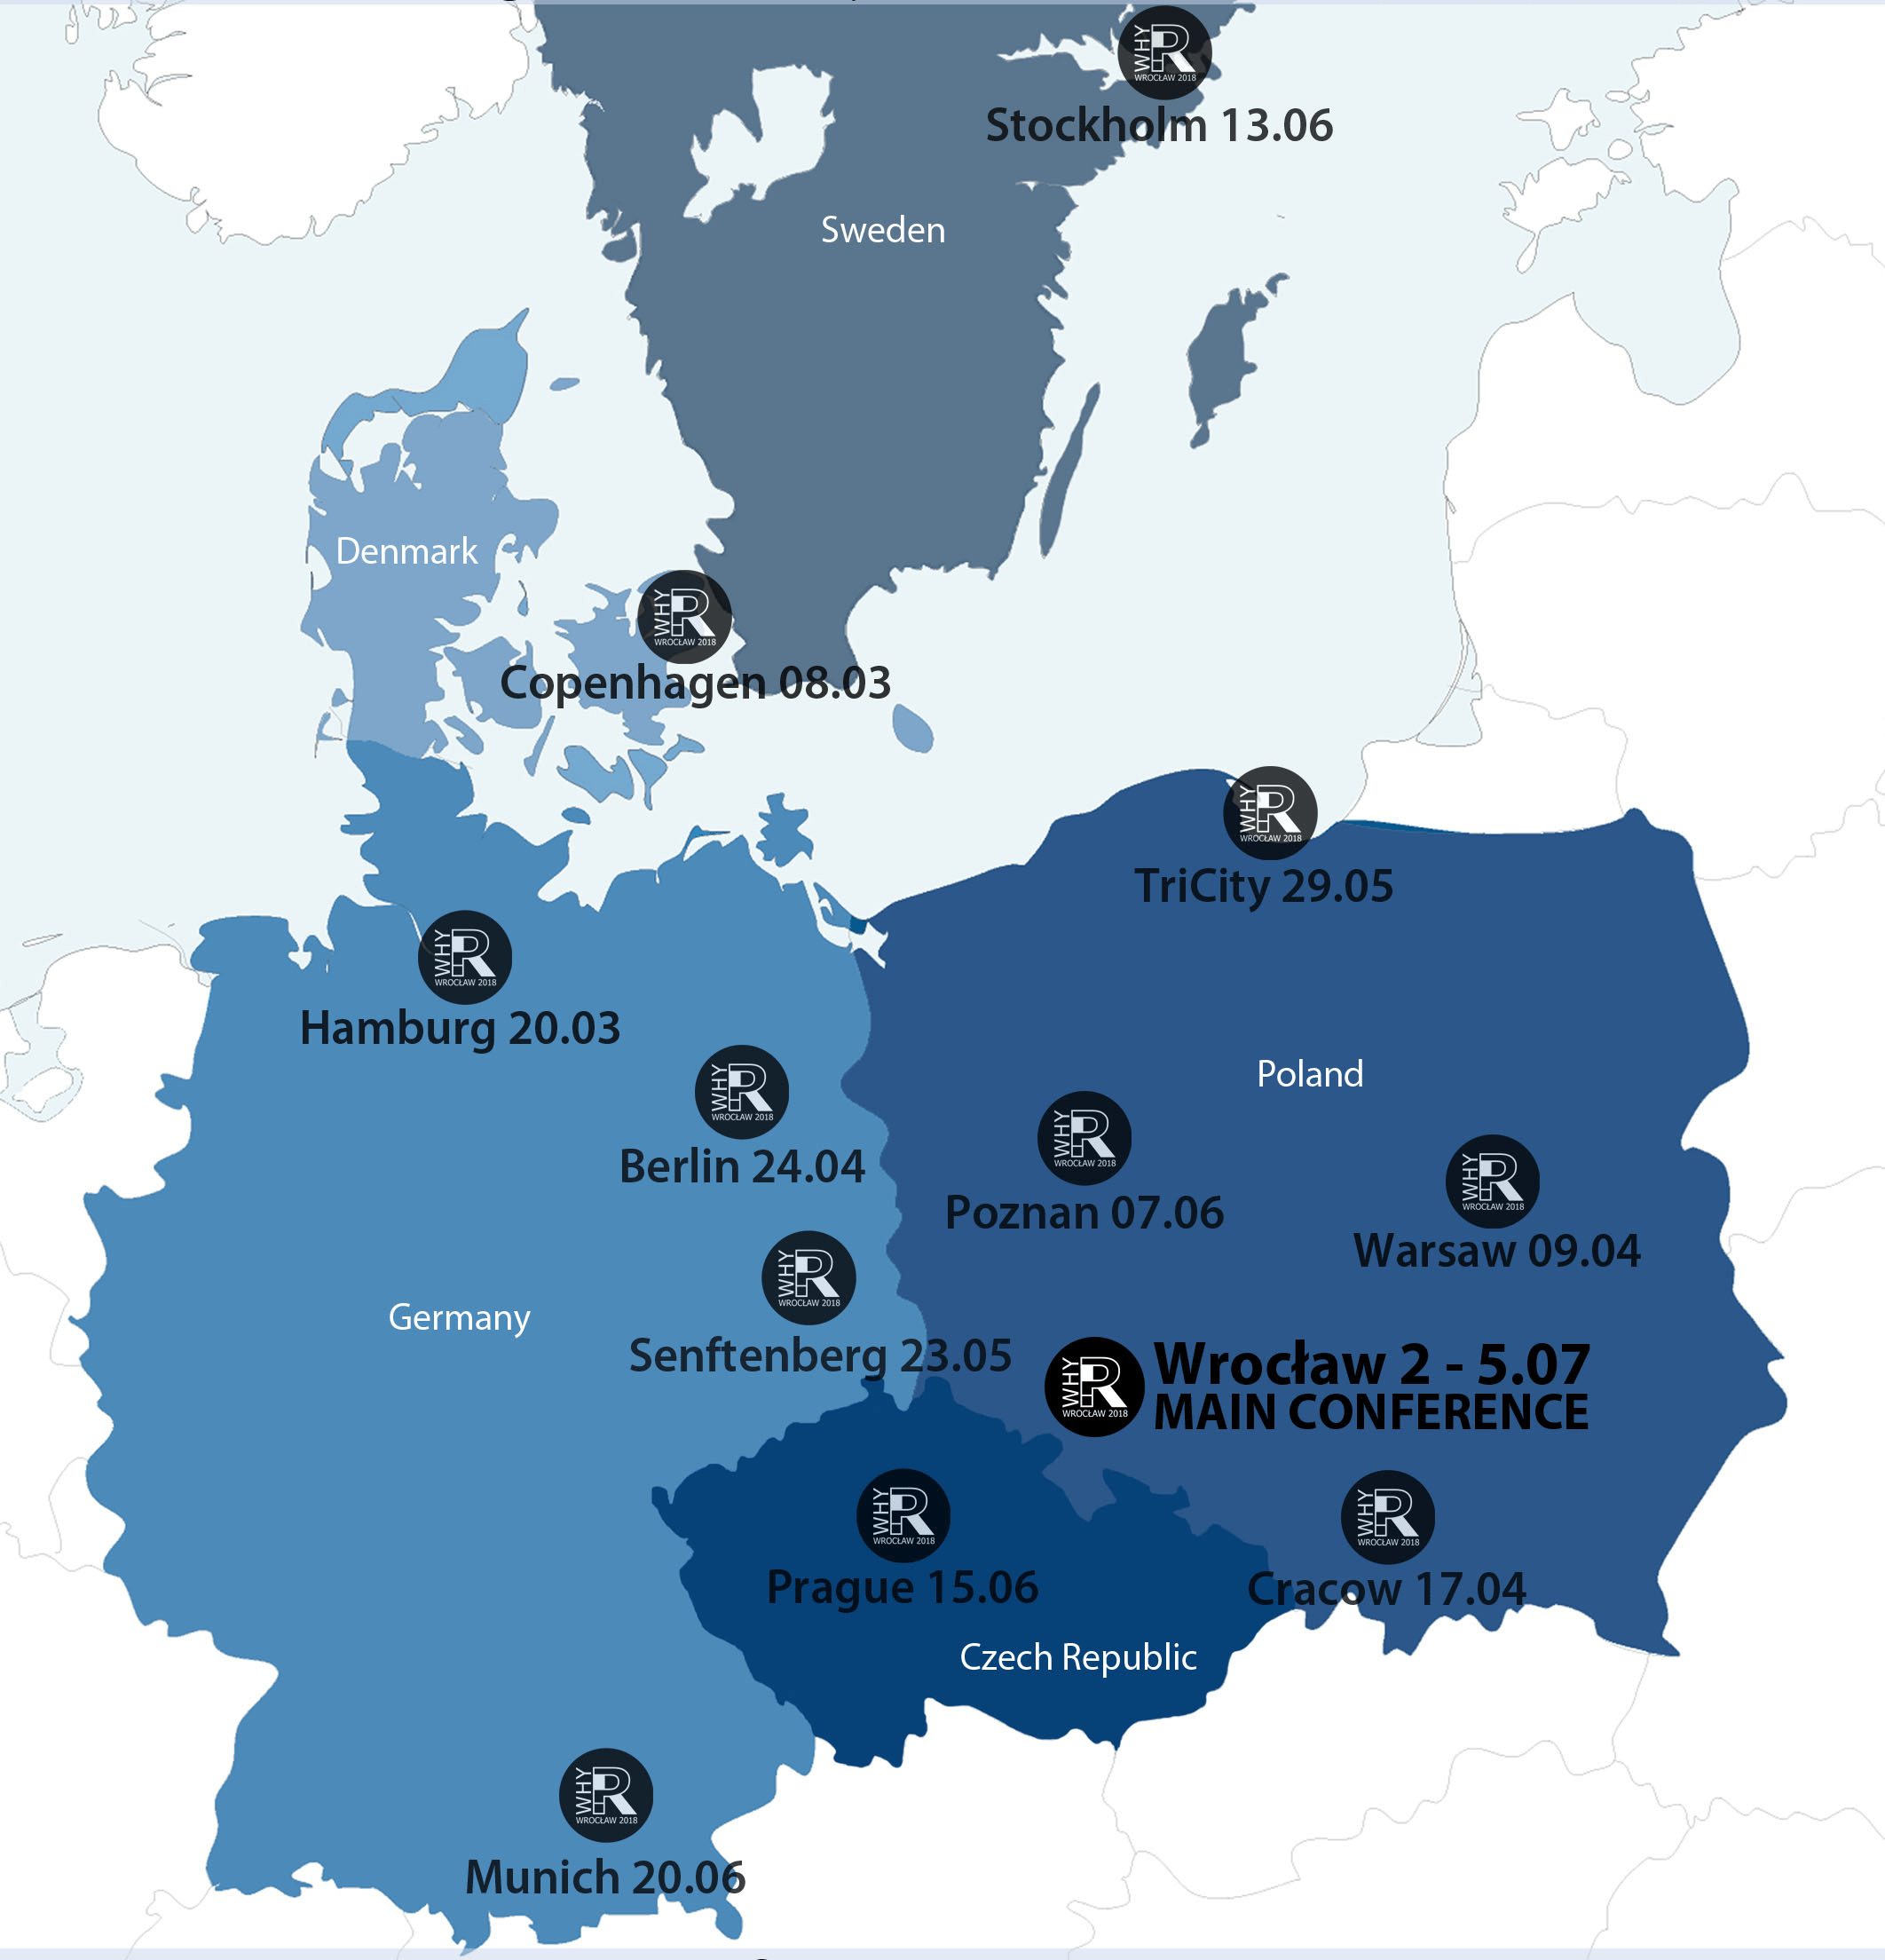
\includegraphics[width=0.65\columnwidth]{premeetings}
  \caption{Locations and dates of the \emph{Why R?} 2018 main conference event and 11 \emph{Why R?}-branded pre-meetings.}
  \label{figure:premeetings}
\end{figure}

\section{Conference program}

The format of the conference was aimed at exposing participants to R language recent developments as well as a wide range of application examples. It consisted of workshops, invited talks, field-specific series of talks, lighting-talks, special interest groups and a full-day programming hackathon. 

~\\ The conference program had a strong focus on machine learning techniques and applications, with \pkg{mlr} \citep{mlr} R package -- an interface to a large number of classification and regression methods -- being emphasized in a  number of presentations, as well as employed during workshops and the hackathon provided by the \pkg{mlr} team. The scope of conference program included statistical methodology, data visualization, R code performance,  building products based on data analyses and R role in academia / industry. 

~\\ The event offered extensive networking opportunities. The cocktail party was held at the conference venue on the 2nd conference day. In addition, convenient location in the close proximity of the old town market square facilitated many informal gatherings that were happening each conference day.

\section{\emph{Why R?} Pre-meetings}

The novel idea of pre-meetings has proved to be successful in popularizing \emph{Why R?} conference in the international community of R users. Eleven pre-meetings took place in Czech Republic, Denmark, Germany, Poland and Sweden in the run-up to the \emph{Why R?} main event. 
The pre-meetings either constituted a part of another conference, one day-long workshop and discussion event or a meeting of a local R user group. 

~\\ As  R provides a versatile framework for reproducible research in different scientific domains \citep{gentleman_statistical_2007,gandrud_reproducible_2013,leeper_archiving_2014,liu_r_2014,rodiger_r_2015}, we considered the \emph{Why R?} pre-meetings as a great opportunity to convey and popularize R as an analytics tool in groups of professionals from different fields. The pre-meeting held at International Biotechnology Innovation Days (\emph{IBID}), an open-access conference held 23-25 May, 2018 at the Brandenburg University of Technology Cottbus - Senftenberg (Senftenberg, Germany)\footnote{\url{http://web.archive.org/web/20180701084524/https://ibid-2018.b2match.io/}} is an example where the R came in close contact with scientist from other domains. \emph{IBID} brought together specialists and experts in the fields of bioanalytics, biomedical and translational research, autoimmune diagnostics, digitalization and engineering; hence it posed an excellent platform to promote R and \emph{Why R?} 2018 conference.  

\section{Workshops}

\emph{Why R?} 2018 conference had a wide portfolio of workshops:

\begin{itemize}
  \item \textbf{Maps in R} by Piotr Sobczyk (OLX Group). Piotr showed how to create spatial data visualization efficiently in the R. He gave a plenty of tips to follow, pitfalls to avoid and a number of useful hacks. Starting from a basic plot function, he covered the usage of \pkg{ggplot2} as well as R packages that use interactive javascript libraries to prepare data reports.
    \item \textbf{iDash - Make your R slides awesome with \pkg{xaringan}} by Miko\l{}aj Olszewski (iDash) and Mikołaj Bogucki (iDash). The workshop introduced the \pkg{xaringan} \citep{xie_xaringan:_2018} package -- an alternative approach to preparing a slide deck. \pkg{xaringan} allows customizing each slide entirely and previewing slides dynamically in RStudio; moreover, the export of the slide deck (natively in HTML) to a pixel-perfect PDF is fairly easy. As \pkg{xaringan} also uses RMarkdown, it allows for reproducible results. 
    \item \textbf{Jumping Rivers - Shiny Basics} and \textbf{Advanced Shiny} by Roman Popat (Jumping Rivers). The instructor Roman Popat from Jumping Rivers conducted two workshops. In first (Shiny Basics), he gave an introduction to creating interactive visualizations of data using Shiny. Here, participants learned how to use \pkg{rmarkdown} and \pkg{htmlwidgets}, input and output bindings to interact with R data structures, input widgets and render functions to create complete page layouts using shiny and shiny dashboard. The advanced Shiny workshop explored how to add functionality to shiny apps using javascript packages and code. In particular, it was showed how one might deal with routines in a Shiny application that take a long time to run and how to provide a good experience for simultaneous users of an app. Finally, the instructor showed how to create a standalone web server API to the R code and how to integrate the use of it into a Shiny application using the \pkg{plumber} \citep{technology_plumber:_2018} package.
    \item \textbf{DALEX - Descriptive mAchine Learning EXplanations} by Mateusz Staniak(Uniwersytet Wroc\l{}awski). THe workshop covered tools for exploration, validation and explanation of complex machine learning models. The packages explored in this workshop include \pkg{mlr} \citep{mlr}, \pkg{DALEX} \citep{biecek_dalex:_2018}, \pkg{live} \citep{live}, \pkg{FactorMerger} \citep{FactorMerger}, \pkg{archivist} \citep{archivist}, \pkg{pdp} \citep{pdp} and \pkg{ALEPlot} \citep{apley_aleplot:_2018}.
    \item \textbf{Constructing scales from survey questions} by Tomasz \.{Z}\'{o}\l{}tak (Educational Research Institute in Warsaw, Poland). Tomasz showed how to create scales based on sets of categorical variables using Categorical Exploratory/Confirmatory Factor Analysis (CEFA / CCFA) and IRT models. He used models with bi-factor rotation to deal with different forms of asking questions and corrected for differences in a style of answering questions asked using a Likert scale. In addition, it was showed how to correct self-assessment knowledge/skill indicators using fake items.
    \item \textbf{From RS data to knowledge – Remote Sensing in R} by Bart\l{}omiej Kraszewski (Forest Research Institute in XXX). Remote sensing data from different sensors is a rich source of information for studying the natural environment, natural phenomena and monitoring some extreme phenomena, such as floods. Bart\l{}omiej presented R language packages that can be used to work with remote sensing data. These included (a) for geographic information system analysis: \pkg{rgdal} \citep{bivand_rgdal:_2018}, \pkg{rgeos} \citep{bivand_rgeos:_2018} and \pkg{sf} \citep{pebesma_sf:_2018}; (b) for raster data processing: \pkg{raster} \citep{hijmans_raster:_2017}; (c)  for Airborne LaserScanning data processing:  the \pkg{lidR} \citep{roussel_lidr:_2018} package. 
    \item \textbf{Introduction to Deep Learning with Keras in R} by Micha\l{} Maj (Appsilon Data Science). The workshop covered many important aspects of Deep Learning with the Keras in R, including sequential model building, performing data ingestion and using pre-trained models and performing fine-tuning. The  \pkg{keras} \citep{allaire_keras:_2018} R package was explored. 
\end{itemize}


\section{Invited talks}

The invited talks topics included domain knowledge from statistics, computer science, natural sciences and economics. The speakers list presents as follows: 

\begin{itemize}
    \item Tomasz Niedzielski (University of Wroclaw):  \textit{Forecasting streamflow using the HydroProg system developed in R},
    \item Daria Szmur\l{}o (McKinsey \& Company): \textit{The age of automation -- What does it mean for data scientists?},
    \item Agnieszka Suchwa\l{}ko (Wroclaw University of Technology): \textit{Project evolution -- from university to commerce},
    \item Bernd Bischl (Ludwig-Maximilians-University of Munich): \textit{Machine learning in R},
    \item Artur Suchwa\l{}ko (QuantUp): \textit{A business view on predictive modeling: goals, assumptions, implementation},
    \item Maciej Eder (Institute of Polish Language): \textit{New advances in text mining: exploring word embeddings},
    \item Thomas Petzoldt (Dresden University of Technology): \textit{Simulation of dynamic models in R},
    \item Leon Eyrich Jessen (Technical University of Denmark): \textit{Deep Learning with R using TensorFlow}.
\end{itemize}

%% @MKaras: I think it would be great to add presentation titles to the above list. I could not find the list quickly, however. 

\section{Special Interest Groups}

Three Special Interest Groups were organized to facilitate topic-specific discussion between conference participants.

\begin{itemize}
\item  \textbf{Diversity in Data Science}, moderated by R-Ladies Warsaw, aimed to discuss boosting the diversity of R community and inspire members of affinity groups to pursue careers in data science. 
\item \textbf{The Career planning in data science}, moderated by Artur Suchwa\l{}ko (QuantUp) and Marcin Kosi\'n{}ski (Why R? Foundation), gave participants a chance to learn from experienced R enthusiasts about their career paths. 
\item \textbf{Teaching of data science}, moderated by Leon Eyrich Jessen (Technical University of Denmark) and Stefan R\"odiger (Brandenburg Technical University Cottbus-Senftenberg), gathered data science experts from academia an industry  to share their experiences and discuss challenges and solutions in teaching different concepts of data science. 
\end{itemize}

\section{Conference organizers}

The quality of the scientific program of the conference was the achievement of Marcin Kosi\'{n}ski, Alicja Gosiewska, Aleksandra Grudzi\k{a}\.{z}, Malte Grosser, Andrej-Nikolai Spiess, Przemys\l{}aw Gagat, Joanna Szyda, Pawe\l{} Mackiewicz, Bartosz S\k{e}kiewicz, Przemys\l{}aw Biecek, Piotr Sobczyk, Marta Kara\'{s}, Marcin Krzystanek, Marcin \L{}ukaszewicz, Agnieszka Borsuk - De Moor, Jaros\l{}aw Chilimoniuk, Micha\l{} Maj and Micha\l{} Kurtys. The organization was in the hands of Micha\l{} Burdukiewicz (chair).

The organizers want to acknowledge R user groups from Berlin, Copenhagen, Cracow, Hamburg, Munich, Poznan, Prague, Stockholm, TriCity, Wroclaw and Warsaw. 

\section{Acknowledgements}

We would like to say thank you to all the sponsors, the University of Wroc\l{}aw, Wroc\l{}aw Center of Biotechnology Consortium, the local organizers of the pre-meetings, the \pkg{mlr} team and student helpers.

\section{Additional information}

\textbf{\emph{Why R?} 2018 website} \url{http://whyr.pl/2018}
\newline
\textbf{Corporate sponsors}: McKinsey \& Company, Wroc\l{}aw Center for Biotechnology, KRUK S.A., iDash s.c., R Consortium, WLOG Solutions, Jumping Rivers Ltd., RStudio, Inc., Analyx\textregistered GmbH and Pearson IOKI.



\bibliography{burdukiewicz}

\address{Micha\l{} Burdukiewicz\\
  Warsaw University of Technology, Why R? Foundation\\
  Pl. Politechniki 1, 00-661 Warsaw\\
  Poland\\}
\email{michalburdukiewicz@gmail.com}

\address{Marta Karas\\
  Johns Hopkins Bloomberg School of Public Health\\
  615 N Wolfe St Rm E3527\\
  Baltimore, MD \\ 
  USA\\}
\email{marta.karass@gmail.com}

\address{Leon Eyrich Jessen\\
  Technical University of Denmark\\
   Anker Engelunds Vej 1, 2800 Kgs. Lyngby, Denmark\\
  Denmark\\}
\email{author1@work}

\address{Marcin Kosi\'{n}ski\\
  Gradient Metrics, Why R? Foundation\\
  Warsaw\\
  Poland\\}
\email{m.p.kosinski@gmail.com}

\address{Bernd Bischl\\
  Ludwig Maximilian University of Munich\\
  Ludwigstraße 33, München\\
  Germany\\}
\email{bernd\_bischl@gmx.net}

\address{Stefan R\"odiger\\
  Brandenburg University of Technology Cottbus--Senftenberg\\
  Universit\"atsplatz 1, Senftenberg\\
  Germany\\}
\email{stefan.roediger@b-tu.de}

